% Generated by book/tools/notebook_to_tex.py. Do not edit by hand.

\chapter[작은 Diffusion LM 입문]{작은 Diffusion LM 입문: 병렬 Denoise 생성}

\label{ch:32}

\markboth{작은 Diffusion LM 입문}{작은 Diffusion LM 입문}

\chaptermeta{32_diffusion_intro/32_diffusion_intro.ipynb}{https://colab.research.google.com/github/yoon-gu/neuqes-101/blob/master/32_diffusion_intro/32_diffusion_intro.ipynb}{작은 BERT-style masked LM을 from scratch로 학습하고 전부 [MASK]인 캔버스에서 병렬 denoise로 영어 동화를 생성}



\index{1diffusion LM@diffusion LM}

\index{1masked diffusion@masked diffusion}

\index{1absorbing mask diffusion@absorbing mask diffusion}

\index{1parallel denoising@parallel denoising}

\index{1BertForMaskedLM@BertForMaskedLM}

\index{1ByteLevel BPE@ByteLevel BPE}

\index{1DiffusionCollator@DiffusionCollator}

\index{1confidence remasking@confidence remasking}

\index{1time weighted CE@time weighted CE}

\index{0병렬 denoise@병렬 denoise}

\index{0마스크 diffusion@마스크 diffusion}

\index{0가변 마스킹@가변 마스킹}

\index{0빈 캔버스 생성@빈 캔버스 생성}

\index{0시간 가중 손실@시간 가중 손실}



\section{작은 mask-diffusion LM 직접 만들기 --- 가변 마스킹과 병렬 denoise}

Phase 5 의 첫 장. \ref{ch:24}--\ref{ch:31}장까지 다룬 \textbf{GPT (decoder, autoregressive, 왼\(\to\)오 순차 생성)} 패러다임에서, 이번엔 \textbf{Diffusion LM (encoder/bidirectional, masked-denoise, 문장 전체를 병렬로 생성)} 패러다임으로 전환합니다.

학습이 끝나면 전부 \texttt{{[}MASK{]}} 인 빈 캔버스에서 시작해, 왼\(\to\)오가 아니라 \textbf{병렬로} 토큰을 채워가며 영어 동화를 만들어냅니다.

\begin{quote}
\emph{“Once upon a time, there was a boy named Timmy. He had found a big toy ball in the park. He went to a big house with his toys. He liked to play with him.”}
\end{quote}

핵심 한 줄: \textbf{BERT MLM (\ref{ch:20}--\ref{ch:23}장) 의 \emph{고정 15\% 마스킹} 을 \emph{0-100\% 가변 마스킹} 으로 일반화하고, 한 번에 복원하는 대신 \emph{여러 번 반복 denoise} 하면 그게 generation 입니다.} \ref{ch:01}장부터 추적해 온 \emph{마스킹 + 토크나이저} 시각이 여기서 클라이맥스에 도달합니다 --- 가려서 맞히던 BERT 가, 가리는 비율을 끝까지 밀어붙이면 \emph{무에서 문장을 만들어내는 생성 모델} 이 됩니다.

작은 BERT-style 모델을 \emph{random init} 으로 from scratch 띄우고, \textbf{TinyStories} 로 \emph{가변 마스킹 denoising} 목표로 학습 \(\to\) reverse process (전부 \texttt{{[}MASK{]}} 에서 시작해 반복 denoise) 로 텍스트를 \emph{왼\(\to\)오가 아닌 병렬} 로 생성하는 과정을 직접 눈으로 봅니다.

\textbf{환경}: Google Colab \textbf{T4 GPU 필수}. \textbf{예상 소요}: 약 25분 (데이터·토큰화 약 5분 + 학습 약 20분 + 생성·궤적).

\begin{center}\rule{0.5\linewidth}{0.5pt}\end{center}

\section{학습 흐름}

\begin{enumerate}
\def\labelenumi{\arabic{enumi}.}
\tightlist
\item
  \textbf{변화 추적표 + Phase 전환 도입부} --- Autoregressive (GPT) \(\to\) Diffusion 큰 그림
\item
  \textbf{변경점} --- 생성 방식 (순차 \(\to\) 병렬 denoise), attention (causal \(\to\) bidirectional), 마스킹 (고정 15\% \(\to\) 가변 0-100\%)
\item
  \textbf{Loss} --- masked-diffusion denoising loss. MLM 의 CE 를 \emph{가변 마스킹 비율 t} 로 일반화 + \inlinecode{1/t} 재가중
\item
  \textbf{마스킹 thread 클라이맥스} --- BERT 의 \emph{고정 15\%} vs diffusion 의 \emph{가변 0-100\%}. 같은 \inlinecode{-100} 트릭
\item
  \textbf{토크나이저 노트} --- 작은 모델엔 작은 vocab (ByteLevel BPE 2048 직접 학습 + \texttt{{[}MASK{]}})
\item
  \textbf{실습}: TinyStories \(\to\) 작은 BERT-style 모델 \(\to\) 가변 마스킹 denoising 학습
\item
  \textbf{Reverse process generation} --- 전부 \texttt{{[}MASK{]}} 에서 반복 denoise. 마스크가 \emph{병렬로} 단어로 채워지는 궤적 직접 관찰
\item
  \textbf{변형}: denoise step 수 비교 (1 / 4 / 16 / 32), 조건부 생성 (prompt 고정)
\item
  \textbf{AR vs Diffusion 비교} --- \ref{ch:24}장 (GPT) 와 나란히. 33장 (샘플러)·34장 (한국어) 예고
\item
  \textbf{등장 라이브러리} / \textbf{체크포인트} / \textbf{FAQ} (답변 포함)
\end{enumerate}

\begin{center}\rule{0.5\linewidth}{0.5pt}\end{center}

\begin{quote}
\textbf{사전 학습 자료}: \ref{ch:20}--\ref{ch:23}장 (BERT MLM 사전학습 --- 고정 15\% 마스킹), \ref{ch:24}장 (GPT from scratch --- autoregressive generation). 본 장은 \emph{둘을 잇습니다} --- BERT 의 \emph{마스킹-복원} 메커니즘을 \ref{ch:24}장의 \emph{generation} 목적에 다시 씁니다. 다른 점은 \emph{마스킹 비율을 0-100\% 로 일반화} 하고 \emph{복원을 여러 번 반복} 한다는 것뿐.
\end{quote}



\section{변화 추적표}

\begin{booktable}{32장 변화 추적표 표}{tab:ch32-01}
\begin{adjustbox}{max width=\textwidth}
\begin{tabular}{@{}lllllll@{}}
\toprule
Ch & 모델 & 토크나이저 & 데이터 & Output Head & 생성/학습 방식 & Loss \\
\midrule

20 & 작은 BERT (영어, scratch) & \inlinecode{bert-base-uncased} (가져옴) & Wikitext-103 & MLM head & 고정 15\% 마스킹-복원 & \inlinecode{CrossEntropyLoss} (masked 15\%) \\
24 & 작은 GPT2 (직접, scratch) & BPE (직접 학습) & TinyStories & \inlinecode{Linear(H,\ V)} & autoregressive (왼\(\to\)오 순차) & \inlinecode{CrossEntropyLoss} (next-token) \\
31 & SFT base + GRPO & BBPE & verifiable-reward & \inlinecode{Linear(H,\ V)} + group adv. & autoregressive + RL & \inlinecode{GRPO\ loss} \\
\textbf{32 \(\leftarrow\) 여기} & \textbf{작은 BERT-style (직접, scratch)} & \textbf{ByteLevel BPE 2048 (직접 학습 + \texttt{{[}MASK{]}})} & \textbf{TinyStories} & \textbf{\inlinecode{Linear(H,\ V)}} & \textbf{parallel denoise (가변 마스킹 + 반복 복원)} & \textbf{masked-diffusion denoising loss (\inlinecode{1/t} 재가중)} \\
33 (다음) & MDLM (170M) / DiffuGPT (124M) 사전학습 & (각 모델 토크나이저) & 영어 사전학습 추론 시연 & \inlinecode{Linear(H,\ V)} & parallel denoise (추론만) & --- \\
\bottomrule
\end{tabular}
\end{adjustbox}
\end{booktable}

전체 장 표는 \href{https://github.com/yoon-gu/neuqes-101\#챕터별-변화추적표}{루트 README} 를 참고하세요.

\begin{center}\rule{0.5\linewidth}{0.5pt}\end{center}

\section{\texorpdfstring{Phase 전환 --- Autoregressive (GPT) \(\to\) Diffusion LM}{Phase 전환 --- Autoregressive (GPT) \textbackslash to Diffusion LM}}

\ref{ch:24}--\ref{ch:31}장의 GPT 장들이 \emph{decoder + next-token 예측 + 왼\(\to\)오 순차 생성} 패러다임이라면, Phase 5 (32-34장) 는 \emph{encoder/bidirectional + masked-denoise + 문장 전체 병렬 생성} 패러다임입니다. 본 장이 그 출발점.

\begin{booktable}{32장 Phase 전환 - Autoregressive (GPT) \textbackslash to Diffusion LM 표}{tab:ch32-02}
\begin{adjustbox}{max width=\textwidth}
\begin{tabular}{@{}lll@{}}
\toprule
축 & Phase 4 (GPT, \ref{ch:24}--\ref{ch:31}장) & \textbf{Phase 5 (Diffusion, 32-34장)} \\
\midrule

attention & Causal (과거만 봄) & \textbf{Bidirectional (양방향 다 봄)} \\
학습 목표 & next-token 예측 & \textbf{가변 마스킹 denoising} \\
생성 순서 & 왼\(\to\)오 \emph{한 토큰씩 순차} & \textbf{문장 전체를 \emph{동시에} 여러 번 denoise} \\
생성 step 수 & 토큰 수 = step 수 (길면 느림) & \textbf{step 수를 \emph{자유롭게 조절} (4 / 16 / 32 ...)} \\
출발 상태 & prompt 토큰들 & \textbf{전부 \texttt{{[}MASK{]}} (무에서 시작)} \\
본체 계보 & GPT (\ref{ch:24}장) & \textbf{BERT (\ref{ch:20}장)} --- MLM 을 일반화 \\
\bottomrule
\end{tabular}
\end{adjustbox}
\end{booktable}

\begin{quote}
\textbf{핵심 직관}: GPT 가 \emph{왼쪽부터 한 글자씩 받아쓰기} 라면, diffusion 은 \emph{흐릿한 전체 그림을 여러 번 선명하게 다듬기} 입니다. 이미지 생성에서 노이즈를 점점 걷어내듯, 텍스트에서는 \texttt{{[}MASK{]}} 를 점점 진짜 단어로 바꿔 갑니다. 본 장은 그 메커니즘을 \emph{작은 모델로 직접 구현} 해 봅니다. 33장 (MDLM 170M / DiffuGPT 124M 사전학습) 이 \emph{같은 원리의, 충분한 규모로 학습된 실전 모델} 입니다.
\end{quote}



\section{변경점: \ref{ch:31}장 대비}

\begin{booktable}{32장 변경점 요약}{tab:ch32-03}
\begin{adjustbox}{max width=\textwidth}
\begin{tabular}{@{}lll@{}}
\toprule
축 & \ref{ch:24}--\ref{ch:31}장 (GPT, autoregressive) & 32장 (Diffusion LM) \\
\midrule

\textbf{생성 방식} & next-token, 왼\(\to\)오 \emph{순차} & \textbf{masked-denoise, 문장 전체 \emph{병렬}} \(\leftarrow\) \emph{Phase 전환의 핵심} \\
attention & Causal (\inlinecode{GPT2LMHeadModel}) & \textbf{Bidirectional (\inlinecode{BertForMaskedLM} 계열)} \\
학습 목표 & \inlinecode{CrossEntropyLoss} (next-token, 거의 모든 자리) & \textbf{masked-diffusion loss (가변 비율 \inlinecode{t} 마스킹 + \inlinecode{1/t} 재가중)} \\
마스킹 & 없음 (causal mask 가 미래 차단) & \textbf{입력 토큰을 \inlinecode{t} 비율로 \texttt{{[}MASK{]}} 치환} \\
토크나이저 & BPE (GPT 계열) & \textbf{ByteLevel BPE 2048 직접 학습 + \texttt{{[}MASK{]}}} \\
생성 출발 & prompt 토큰 & \textbf{전부 \texttt{{[}MASK{]}} 인 시퀀스} \\
생성 step & 토큰 길이 만큼 & \textbf{임의 step 수 (속도-품질 trade-off 조절 가능)} \\
\bottomrule
\end{tabular}
\end{adjustbox}
\end{booktable}

\begin{quote}
\textbf{변경점이 한꺼번에 많은 이유} --- Phase 가 바뀌는 \emph{전환 장} 라 \emph{축 자체} 가 새로 정의됩니다. 하지만 본질은 \emph{\ref{ch:20}장의 BERT MLM 을 재활용} 한 것 --- \emph{bidirectional + 마스킹-복원} 은 이미 다 배운 메커니즘이고, \emph{마스킹 비율을 가변} 으로 만들고 \emph{복원을 반복} 한 것만 새롭습니다. 다음 두 장은 다시 \emph{한 가지씩} 만 바뀝니다 --- \textbf{33장: 샘플러를 바꿔 생성 품질을 끌어올리고, 34장: 한국어로 확장}합니다.
\end{quote}



\section{Loss --- masked-diffusion denoising loss}

BERT MLM 의 CrossEntropyLoss 와 \emph{뼈대는 같습니다} --- 가려진 자리의 정답 토큰을 맞히는 CE. 다른 점은 두 가지:

\begin{enumerate}
\def\labelenumi{\arabic{enumi}.}
\tightlist
\item
  마스킹 비율이 \emph{고정 15\%} 가 아니라 \emph{매 샘플마다 \(t \sim U(0, 1)\) 로 뽑은 가변 비율}
\item
  비율 \(t\) 만큼 가렸으니, loss 를 \emph{\(1/t\) 로 재가중} 해 \emph{어떤 마스킹 비율이든 공정하게} 평균
\end{enumerate}

\subsection{수식}

깨끗한 토큰 시퀀스 \(x_0 = (x_1, \dots, x_L)\) 에 대해, 비율 \(t\) 를 뽑고 각 토큰을 \emph{독립적으로 확률 \(t\)} 로 \texttt{{[}MASK{]}} 치환해 \(x_t\) 를 만듭니다. 모델은 \(x_t\) 전체를 보고 \emph{가려진 자리} 의 원본 토큰을 예측:

\begin{equation}
\label{eq:ch32-01}
L = \mathbb{E}_{t \sim U(0,1)} \left[ \frac{1}{t} \cdot \frac{1}{L} \sum_{i:\, x_t^{(i)} = \inlinecode{[MASK]}} -\log P_\theta\!\left(x_0^{(i)} \mid x_t\right) \right]
\end{equation}

식~\eqref{eq:ch32-01}은 이 절에서 사용하는 핵심 관계를 정리한 것입니다.

\begin{itemize}
\tightlist
\item
  \(\sum_{i:\, x_t^{(i)}=\inlinecode{[MASK]}}\): \emph{가려진 자리에서만} loss 계산 (\ref{ch:20}--\ref{ch:23}장의 \inlinecode{-100} 트릭과 동일)
\item
  \(1/t\) 재가중: \(t\) 가 작으면 (조금 가림) 가려진 토큰이 적으니 합이 작아지는데, \(1/t\) 로 곱해 \emph{마스킹 비율에 무관} 하게 스케일을 맞춤. 이 재가중 덕분에 \emph{학습 목표가 log-likelihood 의 upper bound} 가 됩니다 (LLaDA / MDLM 의 핵심 항)
\item
  \(t \sim U(0,1)\): 매 step 마다 \emph{다른 난이도} 의 복원 문제를 풀게 함 --- 5\% 만 가린 쉬운 문제부터 95\% 가린 거의-무에서-생성 문제까지
\end{itemize}

\subsection{숫자로 감 잡기 (vocab = 2,048)}

random init 직후 모델은 가려진 자리를 \emph{균등 추측} \(\to\) 정답 확률 \(1/2048\), 토큰당 \(-\log p \approx \ln(2048) = 7.62\).

\begin{booktable}{32장 숫자로 감 잡기 (vocab = 2,048) 표}{tab:ch32-04}
\begin{adjustbox}{max width=\textwidth}
\begin{tabular}{@{}lllll@{}}
\toprule
마스킹 비율 \(t\) & 가린 토큰 수 (L=128) & 가린 자리 합 (\(\approx t L \times 7.62\)) & \(\times \frac{1}{t}\frac{1}{L}\) 후 & 해석 \\
\midrule

0.10 & 약 13 & 약 99 & \textbf{7.62} & 조금 가린 쉬운 복원 \\
0.50 & 약 64 & 약 488 & \textbf{7.62} & 절반 가림 \\
0.90 & 약 115 & 약 877 & \textbf{7.62} & 거의 무에서 생성 \\
\bottomrule
\end{tabular}
\end{adjustbox}
\end{booktable}

\textbf{관전 포인트}:

\begin{itemize}
\tightlist
\item
  \inlinecode{1/t} 재가중 덕분에 \emph{어떤 t 든 baseline loss 가 똑같이 \texttt{ln(vocab)\ \$\textbackslash{}approx\$\ 7.62}} 로 정렬됩니다. 직접 학습한 BPE 2048 의 random baseline \texttt{ln(2048)\ \$\textbackslash{}approx\$\ 7.62} 와 같은 값 --- \emph{마스킹 비율만 일반화} 했지 loss 의 척도는 그대로입니다.
\item
  학습 첫 step loss 가 약 7.6 부근에서 시작해 빠르게 떨어지면 정상. 목표는 약 3.7 부근 (작은 모델 + TinyStories).
\item
  \(t\) 가 1 에 가까울수록 (거의 다 가림) \emph{문맥 정보가 거의 없어} 복원이 어려움 \(\to\) diffusion 생성이 \emph{여러 step 에 나눠} 조금씩 푸는 이유.
\end{itemize}



\section{\texorpdfstring{마스킹 thread 클라이맥스 --- \emph{고정 15\%} (BERT) \(\to\) \emph{가변 0-100\%} (diffusion)}{마스킹 thread 클라이맥스 --- 고정 15\% (BERT) \textbackslash to 가변 0-100\% (diffusion)}}

\ref{ch:01}장부터 \emph{토크나이저와 마스킹} 을 일관되게 추적해 왔습니다. 그 흐름이 여기서 정점에 닿습니다.

\begin{booktable}{32장 마스킹 thread 클라이맥스 - 고정 15\% (BERT) \textbackslash to 가변 0-100\% (diffusion) 표}{tab:ch32-05}
\begin{adjustbox}{max width=\textwidth}
\begin{tabular}{@{}lllll@{}}
\toprule
단계 & 장 & 마스킹 비율 & 복원 횟수 & 용도 \\
\midrule

MLM 사전학습 & \ref{ch:20}장 (영어), \ref{ch:22}장 (한국어) & \textbf{고정 15\%} & 1회 & 표현 학습 (downstream fine-tune 용) \\
GPT CausalLM & \ref{ch:24}--\ref{ch:31}장 & 마스킹 없음 (causal mask) & --- & autoregressive 생성 \\
\textbf{Mask-diffusion} & \textbf{32장 (본 장)} & \textbf{가변 \(t \sim U(0,1)\)} & \textbf{반복 (4-32 step)} & \textbf{병렬 생성} \\
\bottomrule
\end{tabular}
\end{adjustbox}
\end{booktable}

핵심은 \textbf{셋이 모두 같은 \inlinecode{labels\ =\ -100} 트릭} 을 쓴다는 점입니다 --- \emph{가려진 자리만} loss 계산, 나머지는 \inlinecode{-100} 으로 무시. \ref{ch:20}장에서 손에 익힌 그 패턴이 그대로 재등장합니다.

\begin{quote}
\textbf{“가린다” 의 의미가 바뀝니다.} BERT 에서 마스킹은 \emph{표현을 배우기 위한 수단} (15\% 만 살짝 가려 문맥으로 복원). Diffusion 에서 마스킹은 \emph{생성 그 자체} --- 100\% 가린 \texttt{{[}MASK{]}} 시퀀스에서 출발해 한 step 씩 단어를 채우면, 그게 \emph{무에서 문장을 만들어내는 것} 입니다. \textbf{같은 메커니즘, 다른 목적.} 가리는 비율을 끝까지 밀어붙였더니 \emph{복원이 생성이 되었습니다.}
\end{quote}

이 장에서 학습 collator 는 매 배치마다 \(t\) 를 새로 뽑아 \emph{가변 비율} 로 가립니다. \ref{ch:20}장의 \inlinecode{DataCollatorForLanguageModeling(mlm=True,\ mlm\_probability=0.15)} 가 \emph{고정 15\%} 였다면, 여기서는 \emph{직접 만든 가변 collator} 가 \emph{0-100\% 를 매번 다르게} 가립니다.



\section{\texorpdfstring{토크나이저 노트}{토크나이저 노트}}

Diffusion LM 의 주인공 토큰은 \textbf{\texttt{{[}MASK{]}}} 입니다. 전부 \texttt{{[}MASK{]}} 인 빈 캔버스에서 시작해 토큰을 채우는 게 곧 생성이니까요.

그런데 작은 from-scratch 모델에는 \textbf{작은 vocab} 이 중요합니다. \inlinecode{bert-base-uncased} 의 WordPiece 는 vocab 이 30,522 개라, hidden 256 짜리 작은 모델에 그대로 붙이면 임베딩 테이블이 파라미터의 대부분을 잡아먹어 정작 문맥을 배우는 본체에 쓸 용량이 없습니다. 그래서 이 장은 \ref{ch:19}·\ref{ch:24}장처럼 \textbf{TinyStories 코퍼스에 ByteLevel BPE 2048 을 직접 학습} 하고, 거기에 \texttt{{[}PAD{]}}·\texttt{{[}UNK{]}}·\texttt{{[}MASK{]}} 특수 토큰을 더해 씁니다.

\begin{booktable}{32장 토크나이저 노트 표}{tab:ch32-06}
\begin{adjustbox}{max width=\textwidth}
\begin{tabular}{@{}llll@{}}
\toprule
토크나이저 & vocab & \texttt{{[}MASK{]}} & 본 장 적합성 \\
\midrule

WordPiece (\inlinecode{bert-base-uncased}) & 30,522 & 내장 & 작은 모델엔 임베딩 과대 \\
BPE (GPT-2) & 50,257 & 없음 & 별도 추가 필요 \\
\textbf{ByteLevel BPE (직접 학습)} & \textbf{2048} & \textbf{추가} & \textbf{작은 모델에 딱 --- 본 장} \\
\bottomrule
\end{tabular}
\end{adjustbox}
\end{booktable}

\texttt{{[}MASK{]}} 토큰이 \emph{forward process (가리기)} 와 \emph{reverse process (복원/생성)} 양쪽의 핵심입니다.

\begin{quote}
\ref{ch:01}장부터 추적한 \emph{토크나이저 시각} 의 클라이맥스 --- \emph{같은 문장이 어떻게 토큰화되는가} 를 넘어, 이제 \emph{\texttt{{[}MASK{]}} 토큰 자체가 생성의 캔버스} 가 됩니다.
\end{quote}



\section{환경 준비}



\section{TinyStories 데이터 로드}

\ref{ch:24}장 (GPT) 와 \emph{완전히 같은 데이터} --- \inlinecode{roneneldan/TinyStories} (Eldan \& Li 2023, arXiv:2305.07759). GPT-3.5 / GPT-4 가 \emph{4세 어린이 어휘} 로 생성한 짧은 영어 동화. 어휘·문법이 단순해 작은 모델로도 의미 있는 생성이 가능합니다.

\emph{데이터를 \ref{ch:24}장과 동일} 하게 둔 이유: 나중에 \emph{같은 데이터에서 AR (\ref{ch:24}장) vs Diffusion (본 장) 생성 방식만 다른} 비교를 하기 위함입니다.

학습 split 의 처음 \textbf{30,000 stories} 만 사용 (T4 30분 룰 안).



\section{\texorpdfstring{ByteLevel BPE 2048 직접 학습 + \texttt{{[}MASK{]}} 추가}{ByteLevel BPE 2048 직접 학습 + {[}MASK{]} 추가}}

\ref{ch:19}·\ref{ch:24}장처럼 TinyStories 코퍼스에 ByteLevel BPE 를 vocab 2,048 으로 직접 학습하고, \texttt{{[}PAD{]}}·\texttt{{[}UNK{]}}·\texttt{{[}MASK{]}} 특수 토큰을 더해 씁니다. 핵심은 \texttt{{[}MASK{]}} 토큰의 존재 (직접 학습이라 \inlinecode{special\_tokens} 로 명시 추가).



\Needspace{11\baselineskip}
\begin{lstlisting}
from tokenizers import Tokenizer, models, trainers, pre_tokenizers, decoders
from transformers import PreTrainedTokenizerFast
VOCAB = 2048
def corpus_iter(bs=1000):
    for i in range(0, len(raw_train), bs):
        yield raw_train[i:i+bs]["text"]
_tk = Tokenizer(models.BPE(unk_token="[UNK]"))
_tk.pre_tokenizer = pre_tokenizers.ByteLevel(add_prefix_space=True)
_tk.decoder = decoders.ByteLevel()
_tk.train_from_iterator(corpus_iter(), trainer=trainers.BpeTrainer(
    vocab_size=VOCAB, special_tokens=["[PAD]", "[UNK]", "[MASK]"]))
tokenizer = PreTrainedTokenizerFast(tokenizer_object=_tk, pad_token="[PAD]",
                                    unk_token="[UNK]", mask_token="[MASK]")
print(f"vocab_size : {tokenizer.vocab_size}")
print(
    f"[MASK]     : '{tokenizer.mask_token}'  id="
\end{lstlisting}

\noindent\emph{앞뒤 블록은 모두 필요한 라이브러리와 기본 설정을 준비하는 단계입니다. 길이를 나누어 같은 흐름을 단계별로 확인합니다.}

\Needspace{11\baselineskip}
\begin{lstlisting}[firstnumber=17]
    f"{tokenizer.mask_token_id}"
)

import random as _r; _r.seed(0)
sample = "Once upon a time, a little rabbit went to the forest."
enc = tokenizer(sample, add_special_tokens=False)["input_ids"]
md = enc[:]
for i in sorted(_r.sample(range(len(enc)), max(1, len(enc)//3))):
    md[i] = tokenizer.mask_token_id
print("\noriginal :", sample)
print("masked   :", tokenizer.decode(md))
\end{lstlisting}

\noindent\textbf{출력.}
\begin{bookoutputbox}
vocab_size : 2048
[MASK]     : '[MASK]'  id=2

original : Once upon a time, a little rabbit went to the forest.
masked   : [MASK] upon a time[MASK] a[MASK] rabbit went to the forest[MASK]
\end{bookoutputbox}
\par\vspace{0.9em}



\textbf{관전 포인트} --- \texttt{{[}MASK{]}} 가 섞인 시퀀스가 바로 diffusion 의 \emph{중간 상태} \(x_t\) 입니다. 학습은 \emph{가려진 자리를 맞히는 것}, 생성은 \emph{전부 \texttt{{[}MASK{]}} 에서 시작해 반복적으로 채우는 것}. \ref{ch:20}장의 MLM 과 토큰 수준에서는 똑같이 생겼습니다 --- 차이는 \emph{마스킹 비율} 과 \emph{반복 횟수}.



\section{\texorpdfstring{토큰화 + \inlinecode{group\_texts} (고정 길이 블록 스트림)}{토큰화 + group\_texts (고정 길이 블록 스트림)}}

\ref{ch:20}·\ref{ch:24}장과 같은 전처리 패턴 --- 전체 코퍼스를 토큰화해 이어 붙이고 \inlinecode{block\_size=128} 단위로 자릅니다. 특수 토큰 (\texttt{{[}CLS{]}}, \texttt{{[}SEP{]}}) 은 넣지 않고 \emph{순수 텍스트 스트림} 으로 만듭니다 (diffusion 은 문장 전체를 한 캔버스로 다루므로 경계 토큰이 불필요).



\Needspace{11\baselineskip}
\begin{lstlisting}
BLOCK_SIZE = 128

def tokenize_fn(batch):

    return tokenizer(batch["text"], add_special_tokens=False)

tok_train = raw_train.map(
    tokenize_fn,
    batched=True,
    remove_columns=raw_train.column_names,
    desc="tokenize train",
)
tok_val   = raw_val.map(
    tokenize_fn,
    batched=True,
    remove_columns=raw_val.column_names,
\end{lstlisting}

\noindent\emph{앞뒤 블록은 모두 텍스트를 모델 입력 텐서로 바꾸는 단계입니다. 길이를 나누어 같은 흐름을 단계별로 확인합니다.}

\Needspace{11\baselineskip}
\begin{lstlisting}[firstnumber=17]
    desc="tokenize val",
)

def group_texts(batch):
    concatenated = {k: sum(batch[k], []) for k in batch.keys()}
    total_len = len(concatenated["input_ids"])
    total_len = (total_len // BLOCK_SIZE) * BLOCK_SIZE
    return {
        k: [t[i : i + BLOCK_SIZE] for i in range(0, total_len, BLOCK_SIZE)]
        for k, t in concatenated.items()
    }

\end{lstlisting}

\noindent\emph{앞 블록은 텍스트를 모델 입력 텐서로 바꾸는 단계입니다. 이어지는 블록에서는 앞에서 만든 중간 값을 다음 계산으로 넘기는 단계로 넘어갑니다.}

\Needspace{11\baselineskip}
\begin{lstlisting}[firstnumber=29]
lm_train = tok_train.map(
    group_texts,
    batched=True,
    desc="group train",
)
lm_val   = tok_val.map(
    group_texts,
    batched=True,
    desc="group val",
)

lm_train = lm_train.remove_columns([c for c in lm_train.column_names if c != "input_ids"])
lm_val   = lm_val.remove_columns([c for c in lm_val.column_names if c != "input_ids"])

\end{lstlisting}

\noindent\emph{앞 블록은 앞에서 만든 중간 값을 다음 계산으로 넘기는 단계입니다. 이어지는 블록에서는 텍스트를 모델 입력 텐서로 바꾸는 단계로 넘어갑니다.}

\Needspace{11\baselineskip}
\begin{lstlisting}[firstnumber=43]
print(
    f"\ntrain chunks: {len(lm_train):,}  (block_size="
    f"{BLOCK_SIZE})"
)
print(f"val   chunks: {len(lm_val):,}")
print(
    f"approx. train tokens: "
    f"{len(lm_train) * BLOCK_SIZE / 1e6:.2f} M"
)
print("\nfirst chunk decode (first 200 chars):")
print(tokenizer.decode(lm_train[0]["input_ids"])[:200])
\end{lstlisting}

\noindent\textbf{출력.}
\begin{bookoutputbox}
train chunks: 189,030  (block_size=128)
val   chunks: 853
approx. train tokens: 24.20 M

first chunk decode (first 200 chars):
One day, a little girl named Lily found a needle in her room. She knew it w...
\end{bookoutputbox}
\par\vspace{0.9em}



\section{\texorpdfstring{Diffusion collator --- \emph{가변 비율} 마스킹 직접 구현}{Diffusion collator --- 가변 비율 마스킹 직접 구현}}

여기가 BERT MLM 과 갈리는 지점입니다. \ref{ch:20}장은 \inlinecode{DataCollatorForLanguageModeling(mlm\_probability=0.15)} 로 \emph{고정 15\%} 를 가렸지만, diffusion 은 \textbf{매 샘플마다 \(t \sim U(\epsilon, 1)\) 을 뽑아 그 비율로} 가립니다.

\begin{itemize}
\tightlist
\item
  각 토큰을 \emph{독립적으로 확률 \(t\)} 로 \texttt{{[}MASK{]}} 치환 (LLaDA 의 forward process 와 동일)
\item
  \inlinecode{labels}: 가려진 자리는 원본 토큰 id, 나머지는 \inlinecode{-100} (\ref{ch:20}장의 \inlinecode{-100} 트릭 그대로)
\item
  \inlinecode{t}: \(1/t\) 재가중을 위해 샘플별 비율도 함께 반환
\end{itemize}

\inlinecode{add\_special\_tokens=False} 로 토큰화했으므로 시퀀스 안에 특수 토큰이 없어 \emph{모든 자리가 마스킹 가능} 합니다.



\Needspace{11\baselineskip}
\begin{lstlisting}
class DiffusionCollator:
    '''매 배치마다 t ~ U(eps, 1) 을 뽑아 그 비율로 토큰을 [MASK] 치환.'''

    def __init__(self, tokenizer, eps=0.02, seed=42):
        self.mask_id = tokenizer.mask_token_id
        self.eps = eps
        self.gen = torch.Generator().manual_seed(seed)

    def __call__(self, examples):
        ids = torch.tensor(
            [e["input_ids"] for e in examples],
            dtype=torch.long,
        )
        B, L = ids.shape

\end{lstlisting}

\noindent\emph{앞 블록은 텍스트를 모델 입력 텐서로 바꾸는 단계입니다. 이어지는 블록에서는 앞에서 만든 중간 값을 다음 계산으로 넘기는 단계로 넘어갑니다.}

\Needspace{11\baselineskip}
\begin{lstlisting}[firstnumber=16]
        t = torch.rand(
            B,
            generator=self.gen) * (1.0 - self.eps) + self.eps          # (B,,
        )

        mask = torch.rand(B, L, generator=self.gen) < t.unsqueeze(1)
        # (B, L) bool

        no_mask_rows = ~mask.any(dim=1)
\end{lstlisting}

\noindent\emph{앞뒤 블록은 모두 앞에서 만든 중간 값을 다음 계산으로 넘기는 단계입니다. 길이를 나누어 같은 흐름을 단계별로 확인합니다.}

\Needspace{11\baselineskip}
\begin{lstlisting}[firstnumber=25]
        if no_mask_rows.any():
            j = torch.randint(
                0,
                L,
                (int(no_mask_rows.sum()),),
                generator=self.gen,
            )
            mask[no_mask_rows, j] = True

        input_ids = ids.clone()
        input_ids[mask] = self.mask_id
        labels = ids.clone()
        labels[~mask] = -100

\end{lstlisting}

\noindent\emph{앞 블록은 앞에서 만든 중간 값을 다음 계산으로 넘기는 단계입니다. 이어지는 블록에서는 텍스트를 모델 입력 텐서로 바꾸는 단계로 넘어갑니다.}

\Needspace{11\baselineskip}
\begin{lstlisting}[firstnumber=39]
        attention_mask = torch.ones(
            B,
            L,
            dtype=torch.long,
        )
        return {"input_ids": input_ids, "attention_mask": attention_mask,
                "labels": labels, "t": t}

diff_collator = DiffusionCollator(tokenizer)

\end{lstlisting}

\noindent\emph{앞 블록은 텍스트를 모델 입력 텐서로 바꾸는 단계입니다. 이어지는 블록에서는 앞에서 만든 중간 값을 다음 계산으로 넘기는 단계로 넘어갑니다.}

\Needspace{11\baselineskip}
\begin{lstlisting}[firstnumber=49]
print(
    "=== diffusion collator demo (same 2 chunks, masking "
    "ratio varies each call) ==="
)
for trial in range(3):
    batch = diff_collator([lm_train[0], lm_train[1]])
    labels = batch["labels"]
    t = batch["t"]
    for b in range(labels.shape[0]):
        n_masked = (labels[b] != -100).sum().item()
        frac = 100 * n_masked / labels.shape[1]
        print(
            f"trial {trial} | sample {b}: t={t[b]:.3f}  ->  masked {n_masked:>3d}/{labels.shape[1]} ("
            f"{frac:5.1f}%)"
        )
    print()
\end{lstlisting}



\textbf{관전 포인트} --- \ref{ch:20}장 MLM collator 가 \emph{항상 약 15\%} 를 가렸다면, 이 collator 는 \emph{호출마다 0-100\% 사이 아무 값} 으로 가립니다. 같은 chunk 가 어떤 step 엔 5\% 만, 다른 step 엔 90\% 가려진 채 학습됩니다 \(\to\) 모델이 \emph{모든 난이도의 복원} 을 골고루 학습 \(\to\) 생성 시 \emph{어떤 마스킹 비율에서도} denoise 가능.

\begin{quote}
\textbf{\inlinecode{-100} thread}: 가려진 자리만 \inlinecode{labels}, 나머지는 \inlinecode{-100}. \ref{ch:20}장 (MLM 15\%) \(\to\) \ref{ch:28}장 (SFT, prompt 만 \inlinecode{-100}) \(\to\) 본 장 (가변 마스킹) --- 같은 트릭의 세 번째 변주.
\end{quote}



\section{작은 BERT-style 모델 from scratch}

diffusion 의 본체는 \emph{bidirectional encoder} --- 가려진 자리를 \emph{좌·우 양방향 문맥} 으로 복원해야 하니 BERT 계열이 자연스럽습니다. \inlinecode{BertForMaskedLM} 을 \emph{random init} 으로 작게 띄웁니다 (\ref{ch:20}장의 작은 BERT 와 같은 패턴).

\begin{itemize}
\tightlist
\item
  \inlinecode{num\_hidden\_layers=4,\ num\_attention\_heads=4,\ hidden\_size=256} \(\to\) 약 3.79M params (작은 vocab 2048 덕분에 임베딩도 가벼움)
\item
  \inlinecode{max\_position\_embeddings\ =\ BLOCK\_SIZE\ =\ 128}
\item
  MLM head (\inlinecode{Linear(H,\ V)}) 가 \emph{가려진 자리의 토큰 분포} 를 출력 --- 이게 곧 diffusion 의 denoiser
\end{itemize}

\subsection{GPT (\ref{ch:24}장) 와 코드로 갈리는 곳}

\begin{itemize}
\tightlist
\item
  \inlinecode{GPT2LMHeadModel} 이 아니라 \inlinecode{BertForMaskedLM} --- \emph{causal mask 없는 bidirectional attention}
\item
  같은 \inlinecode{from\_pretrained} 없이 \inlinecode{BertForMaskedLM(config)} random init --- \ref{ch:20}·\ref{ch:22}장과 동일
\end{itemize}



\Needspace{11\baselineskip}
\begin{lstlisting}
from transformers import BertConfig, BertForMaskedLM

config = BertConfig(
    vocab_size=tokenizer.vocab_size,
    hidden_size=256,
    num_hidden_layers=4,
    num_attention_heads=4,
    intermediate_size=1024,
    max_position_embeddings=BLOCK_SIZE,
    pad_token_id=tokenizer.pad_token_id,
)

\end{lstlisting}

\noindent\emph{앞 블록은 필요한 라이브러리와 기본 설정을 준비하는 단계입니다. 이어지는 블록에서는 앞에서 만든 중간 값을 다음 계산으로 넘기는 단계로 넘어갑니다.}

\Needspace{11\baselineskip}
\begin{lstlisting}[firstnumber=13]
model = BertForMaskedLM(config).to(device)
n_params = model.num_parameters()
print(f"#params           : {n_params/1e6:.2f} M")
print(f"vocab_size        : {config.vocab_size}")
print(f"\nmodel: {type(model).__name__}")
print(
    f"  - body : "
    f"{type(model.bert).__name__}  (Encoder, bidirectional attention)"
)
print(
    f"  - head : MLM head -> Linear(in={config.hidden_size}, out="
    f"{config.vocab_size})"
)
\end{lstlisting}

\noindent\textbf{출력.}
\begin{bookoutputbox}
#params           : 3.79 M
vocab_size        : 2048

model: BertForMaskedLM
  - body : BertModel  (Encoder, bidirectional attention)
  - head : MLM head -> Linear(in=256, out=2048)
\end{bookoutputbox}
\par\vspace{0.9em}



\section{Reverse process --- 병렬 denoise 생성 함수}

diffusion 생성의 핵심. \textbf{전부 \texttt{{[}MASK{]}} 인 시퀀스에서 시작}해 여러 step 에 걸쳐 점점 진짜 토큰으로 채웁니다 (LLaDA 의 \emph{low-confidence remasking} 방식):

\begin{enumerate}
\def\labelenumi{\arabic{enumi}.}
\tightlist
\item
  현재 \texttt{{[}MASK{]}} 자리들을 모델이 \emph{한꺼번에} 예측 (병렬!)
\item
  각 예측의 \emph{confidence} (softmax 최대 확률) 계산
\item
  \emph{확신 높은} 자리부터 확정, \emph{확신 낮은} 자리는 다시 \texttt{{[}MASK{]}} 로 남김
\item
  스케줄에 따라 남기는 \texttt{{[}MASK{]}} 수를 step 마다 줄여 마지막엔 0개
\end{enumerate}

GPT 의 \emph{왼\(\to\)오 순차} 와 결정적으로 다른 점: \textbf{채우는 순서가 위치가 아니라 confidence 순} --- 문장 중간이나 끝 단어가 앞 단어보다 먼저 확정될 수 있습니다.



\Needspace{11\baselineskip}
\begin{lstlisting}
@torch.no_grad()
def diffusion_generate(active_model, length=64, steps=16, temperature=1.0, top_k=50,
                       prompt_ids=None, record_trajectory=False):
    '''전부 [MASK] 에서 시작해 steps 번 denoise. prompt_ids 를 주면 앞부분 고정 (조건부 생성).

    기본은 sampling (temperature>0). temperature=0 으로 두면 greedy 인데,
    작은 모델 + 전부-[MASK] 출발에서는 greedy 가 최빈 토큰('.')만 뽑는 *collapse* 가 잘 일어나
    sampling 을 기본값으로 둡니다 (아래 한계 노트 참고).'''
    active_model.eval()
    dev = active_model.device
    mask_id = tokenizer.mask_token_id

\end{lstlisting}

\noindent\emph{앞 블록은 텍스트를 모델 입력 텐서로 바꾸는 단계입니다. 이어지는 블록에서는 앞에서 만든 중간 값을 다음 계산으로 넘기는 단계로 넘어갑니다.}

\Needspace{11\baselineskip}
\begin{lstlisting}[firstnumber=13]
    x = torch.full(
        (1, length),
        mask_id,
        dtype=torch.long,
        device=dev,
    )
    fixed = torch.zeros(
        length,
        dtype=torch.bool,
        device=dev,
    )
\end{lstlisting}

\noindent\emph{앞 블록은 앞에서 만든 중간 값을 다음 계산으로 넘기는 단계입니다. 이어지는 블록에서는 모델 출력을 확률이나 예측값으로 바꾸는 단계로 넘어갑니다.}

\Needspace{11\baselineskip}
\begin{lstlisting}[firstnumber=24]
    if prompt_ids is not None:
        p = torch.tensor(prompt_ids[:length], device=dev)
        x[0, :len(p)] = p
        fixed[:len(p)] = True
    n_gen = int((~fixed).sum().item())

    traj = []
    for step in range(steps):
        logits = active_model(input_ids=x).logits[0]
        # (L, V)
        probs = logits.softmax(dim=-1)
        if temperature > 0:
            scaled = logits / temperature
\end{lstlisting}

\noindent\emph{앞 블록은 모델 출력을 확률이나 예측값으로 바꾸는 단계입니다. 이어지는 블록에서는 앞에서 만든 중간 값을 다음 계산으로 넘기는 단계로 넘어갑니다.}

\Needspace{11\baselineskip}
\begin{lstlisting}[firstnumber=37]
            if top_k > 0:
                kth = scaled.topk(top_k, dim=-1).values[:, -1, None]
                scaled = scaled.masked_fill(
                    scaled < kth,
                    float("-inf"),
                )
            pred = torch.multinomial(scaled.softmax(-1), 1).squeeze(-1)
            conf = probs.gather(-1, pred.unsqueeze(-1)).squeeze(-1)
        else:
            conf, pred = probs.max(dim=-1)

        is_mask = (x[0] == mask_id) & (~fixed)

        x_new = torch.where(is_mask, pred, x[0])

\end{lstlisting}

\noindent\emph{앞뒤 블록은 모두 앞에서 만든 중간 값을 다음 계산으로 넘기는 단계입니다. 길이를 나누어 같은 흐름을 단계별로 확인합니다.}

\Needspace{11\baselineskip}
\begin{lstlisting}[firstnumber=52]
        n_remain = int(round(n_gen * (1.0 - (step + 1) / steps)))
        if n_remain > 0:

            conf_masked = conf.clone()
            conf_masked[~is_mask] = float("inf")
            remask_idx = conf_masked.topk(n_remain, largest=False).indices
            x_new[remask_idx] = mask_id

        x[0] = x_new
        if record_trajectory:
            traj.append(x[0].clone())

\end{lstlisting}

\noindent\emph{앞 블록은 앞에서 만든 중간 값을 다음 계산으로 넘기는 단계입니다. 이어지는 블록에서는 텍스트를 모델 입력 텐서로 바꾸는 단계로 넘어갑니다.}

\Needspace{7\baselineskip}
\begin{lstlisting}[firstnumber=64]
    text = tokenizer.decode(
        x[0],
        skip_special_tokens=True,
    )
    return (text, traj) if record_trajectory else text
\end{lstlisting}



\section{\texorpdfstring{학습 \emph{전} denoise - 비교 기준선 (random init baseline)}{학습 전 denoise - 비교 기준선 (random init baseline)}}

학습 전 모델은 가려진 자리를 \emph{균등 추측} 하니, denoise 결과가 \emph{의미 없는 토큰 나열} 이 나옵니다. 학습 후와 나란히 비교하기 위한 기준선 (\ref{ch:20}·\ref{ch:22}장의 \emph{사전학습 전 {[}MASK{]} top-5}, \ref{ch:24}장의 \emph{학습 전 generation} 과 같은 역할).



\textbf{관전 포인트} - 학습 전엔 \emph{영어 문장과 거리가 먼 토큰 나열}. logits 가 random 이라 confidence 순서도 무의미. 학습 후 같은 함수로 다시 생성해 비교하면 \emph{diffusion 학습이 본체에 무엇을 새겼는가} 가 드러납니다.



\section{\texorpdfstring{\inlinecode{Trainer} 로 diffusion 학습 --- \inlinecode{1/t} 재가중 loss}{Trainer 로 diffusion 학습 --- 1/t 재가중 loss}}

BERT/GPT 장들과 같은 \inlinecode{Trainer} 패턴이지만, \emph{loss 를 직접 정의} 합니다. \inlinecode{BertForMaskedLM} 의 기본 loss 는 \emph{가려진 자리 CE 평균} 인데, diffusion 은 거기에 \emph{샘플별 \inlinecode{1/t} 재가중} 을 더해야 합니다 (\inlinecode{compute\_loss} 오버라이드).

\begin{itemize}
\tightlist
\item
  \inlinecode{DiffusionCollator} \(\to\) 매 배치 가변 마스킹 + \inlinecode{t} 반환
\item
  \inlinecode{compute\_loss} \(\to\) 가려진 자리 CE 를 샘플별로 합산해 \inlinecode{1/t} 곱한 뒤 평균
\item
  \inlinecode{max\_steps=30000}, \inlinecode{batch\_size=64}, \inlinecode{fp16=True} - T4 약 19분
\end{itemize}



\compactCodeOmitted{텍스트를 모델 입력 텐서로 바꾸는 단계}

\begin{bookfigurelabel}[H]{32장 diffusion LM 학습 loss와 VRAM 추적}{fig:ch32-training-trace}
\centering
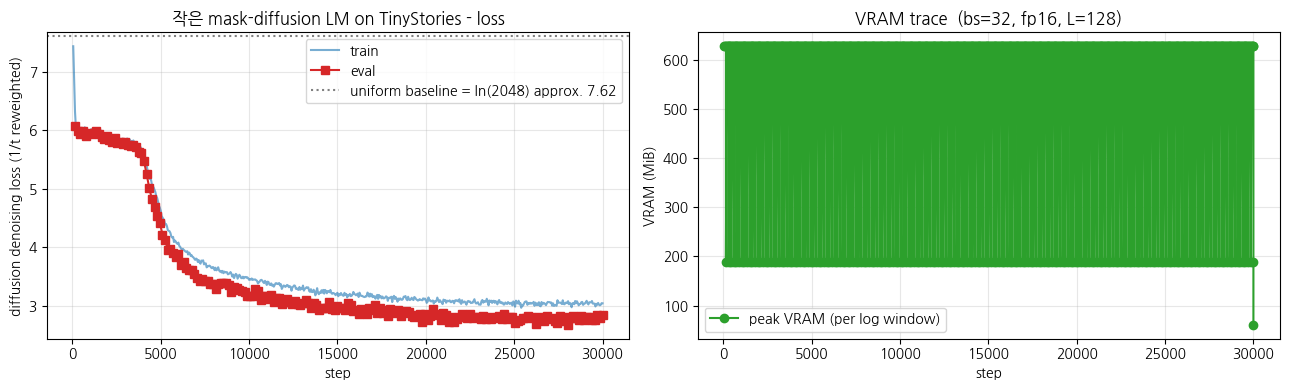
\includegraphics[width=0.86\linewidth]{assets/figures/ch32_training_trace.png}
\end{bookfigurelabel}

\textbf{그림 읽기} --- 그림~\ref{fig:ch32-training-trace}에서 다음 내용을 확인합니다: 32장 diffusion LM 학습 loss와 VRAM 추적. 실행된 노트북에서 저장된 최신 plot 출력이므로, 코드에서 계산한 값이 어떤 평가 지점으로 이어지는지 바로 확인할 수 있습니다.



\textbf{관전 포인트} - \inlinecode{1/t} 재가중 덕분에 첫 step loss 가 약 7.6 (\inlinecode{ln(2048)}) 부근에서 시작 (직접 학습한 BPE 2048 의 random baseline 과 같은 값!). 빠르게 떨어져 30000 step 끝에 \emph{약 3.7} 부근에서 안정화되면 정상. 작은 모델 + TinyStories 라 완벽하진 않지만 \emph{가려진 자리를 문맥으로 복원} 하는 능력이 본체에 새겨집니다.



\section{\texorpdfstring{학습 \emph{후} denoise + 궤적 시각화}{학습 후 denoise + 궤적 시각화}}

같은 \inlinecode{diffusion\_generate} 로 학습 후 생성하고, \textbf{denoise 궤적} (각 step 의 시퀀스) 을 출력해 \emph{마스크가 단어로 채워지는 과정} 을 직접 봅니다. 이게 이 장의 하이라이트 --- GPT 의 왼\(\to\)오 순차와 달리, \emph{문장 전체가 동시에 흐릿하게 떠오르다 선명해지는} 모습.



\Needspace{11\baselineskip}
\begin{lstlisting}
torch.manual_seed(SEED)
text, traj = diffusion_generate(
    model,
    length=40,
    steps=12,
    record_trajectory=True,
)

def render(ids):
    toks = tokenizer.convert_ids_to_tokens(ids.tolist())
    return " ".join("____" if tk == tokenizer.mask_token else tk for tk in toks)

\end{lstlisting}

\noindent\emph{앞뒤 블록은 모두 텍스트를 모델 입력 텐서로 바꾸는 단계입니다. 길이를 나누어 같은 흐름을 단계별로 확인합니다.}

\Needspace{11\baselineskip}
\begin{lstlisting}[firstnumber=13]
print("=" * 78)
print(
    "DENOISE TRAJECTORY  ('____' = still [MASK])  - "
    "filled in parallel, by confidence"
)
print("=" * 78)
n_steps = len(traj)
for step in [0, n_steps // 4, n_steps // 2, 3 * n_steps // 4, n_steps - 1]:
    n_mask = (traj[step] == tokenizer.mask_token_id).sum().item()
    print(
        f"\nstep {step:>2d}/{n_steps-1}  ([MASK] remaining: "
        f"{n_mask:>2d})"
    )
    print("  " + render(traj[step]))

\end{lstlisting}

\noindent\emph{앞 블록은 텍스트를 모델 입력 텐서로 바꾸는 단계입니다. 이어지는 블록에서는 앞에서 만든 중간 값을 다음 계산으로 넘기는 단계로 넘어갑니다.}

\Needspace{5\baselineskip}
\begin{lstlisting}[firstnumber=28]
print("\n" + "=" * 78)
print("FINAL:", text)
\end{lstlisting}

\noindent\textbf{출력.}
\begin{bookoutputbox}
==============================================================================
DENOISE TRAJECTORY ('____' = still [MASK]) - filled in parallel, by confidence
==============================================================================

step  0/11  ([MASK] remaining: 37)
____ ____ ____ ____ ____ ____ ____ ____ ____ . ____ ____ ____ ____ <sp>and...

step  3/11  ([MASK] remaining: 27)
<nl> They <sp>and ____ ____ ____ ____ ____ ____ . <sp>They <sp>likes <sp>to...

step  6/11  ([MASK] remaining: 17)
<nl> They <sp>and ____ . <sp>They ____ ____ ____ . <sp>They <sp>likes <sp>t...

step  9/11  ([MASK] remaining:  7)
<nl> They <sp>and <sp>smile . <sp>They ____ ____ ____ . <sp>They <sp>likes...

...
\end{bookoutputbox}
\par\vspace{0.9em}



\textbf{해석 가이드 - 이게 autoregressive 와 결정적으로 다른 점}

\begin{itemize}
\tightlist
\item
  \textbf{step 0}: 거의 전부 \inlinecode{\_\_\_\_} (\texttt{{[}MASK{]}}). 모델이 \emph{가장 확신하는} 몇 자리만 먼저 채워짐 --- \emph{위치 순서가 아니라 confidence 순서}. 문장 끝/중간 단어가 앞보다 먼저 나타날 수 있음.
\item
  \textbf{중간 step}: 단어들이 \emph{여기저기 동시에} 떠오름. GPT 라면 왼쪽부터 한 칸씩 채워졌을 자리가, diffusion 에선 \emph{전 영역이 함께} 선명해짐.
\item
  \textbf{마지막 step}: 모든 \texttt{{[}MASK{]}} 가 채워진 완성 문장.
\end{itemize}

\begin{quote}
\ref{ch:24}장의 GPT generation 이 \emph{왼\(\to\)오 받아쓰기} 였다면, 여기선 \emph{흐릿한 전체 그림을 반복적으로 다듬기}. 같은 TinyStories 데이터, 같은 “다음 단어가 뭘까” 직관이지만 \emph{생성 메커니즘이 근본적으로 다릅니다.}
\end{quote}



\section{\texorpdfstring{솔직한 이야기 --- 생성은 되지만 \emph{반복} 이 보인다}{솔직한 이야기 --- 생성은 되지만 반복 이 보인다}}

학습이 끝난 모델은 전부 \texttt{{[}MASK{]}} 에서 출발해도 \emph{영어 동화} 를 만들어냅니다 --- 인물·대화·배경이 있는 문장이 병렬 denoise 로 채워집니다. 다만 자세히 읽어 보면 \textbf{같은 조각이 반복} 되는 게 눈에 띕니다.

\begin{quote}
\emph{“Once upon a time, there was a \textbf{a} boy named \textbf{named} Timmy. ... They are happy friends and happy. They are \textbf{to play and play}.”}
\end{quote}

\inlinecode{named\ named}, \inlinecode{was\ a\ was\ a}, \inlinecode{play\ and\ play} 처럼요. 이건 \emph{모델이 잘못 배운 게 아닙니다.} 고정-\(t\)(0.15) 복원 정확도가 0.7 안팎까지 오른, 조건부 구조를 제대로 익힌 모델입니다. 반복의 원인은 \textbf{샘플러} 에 있습니다.

\begin{itemize}
\tightlist
\item
  이 장의 기본 샘플러는 매 step \emph{confidence 가 높은 자리를 채우고 낮은 자리를 다시 \texttt{{[}MASK{]}}} 로 두는 방식인데, 한번 “안전한” 고빈도 토큰(\inlinecode{a}, \inlinecode{the}, 자주 나오는 이름)이 높은 confidence 를 받으면 그 토큰이 거듭 뽑히기 쉽습니다.
\item
  즉 \emph{모델의 확률 분포는 멀쩡한데, 거기서 문장을 어떻게 뽑아내느냐} 가 아직 거친 것입니다.
\end{itemize}

\begin{quote}
그래서 \textbf{다음 33장은 모델은 그대로 두고 샘플러만 바꿉니다} --- carry-over semi-AR + 반복 억제(temperature·top-p·repetition penalty·인접 중복 금지)로 이 반복을 잡아 한결 깔끔한 생성을 얻습니다. 이 장에서 “diffusion 이 글을 만든다”를 확인했다면, 다음 장은 “그 글을 더 잘 뽑아낸다”입니다.
\end{quote}



\section{변형 1 - 조건부 생성 (prompt 고정)}

조건부 생성은 \emph{문맥(prompt)이 있어} unconditional 보다 잘 동작합니다. 작은 모델의 강점 영역.

GPT 의 prompt 에 대응하는 diffusion 버전: \emph{앞부분 토큰을 고정} (절대 마스킹 안 함) 하고 \emph{나머지만} denoise. “Once upon a time” 을 주고 뒤를 채우게 합니다.



\Needspace{11\baselineskip}
\begin{lstlisting}
prompt = "Once upon a time"
prompt_ids = tokenizer(prompt, add_special_tokens=False)["input_ids"]

torch.manual_seed(SEED)
print(f"prompt (fixed): {prompt}")
print("=" * 70)
for i in range(3):
    text = diffusion_generate(
        model,
        length=48,
        steps=16,
        prompt_ids=prompt_ids,
    )
    print(f"\n[sample {i}] {text}")
\end{lstlisting}

\noindent\textbf{출력.}
\begin{bookoutputbox}
prompt (fixed): Once upon a time
======================================================================

[sample 0] Once upon a time, there was a little girl named Lily. She loved...

[sample 1] Once upon a time, there a a little girl named Lily. She loved to...

[sample 2] Once upon a time, there was a little girl named Lily. She was ve...
\end{bookoutputbox}
\par\vspace{0.9em}



\textbf{관전 포인트} - 앞 토큰들이 고정된 채 뒤가 채워집니다. 단, diffusion 은 \emph{양방향} 이라 GPT 와 달리 \emph{prompt 앞이나 중간에 빈칸} 을 두고 채우게 할 수도 있습니다 (infilling) --- autoregressive 가 구조적으로 못 하는 일.



\section{변형 2 - denoise step 수 비교 (속도 - 품질 trade-off)}

diffusion 만의 자유도: \emph{생성 step 수} 를 바꿀 수 있습니다. GPT 는 토큰 수 = step 수로 고정이지만, diffusion 은 \emph{적은 step (빠르지만 거침) \(\leftrightarrow\) 많은 step (느리지만 정교)} 을 조절합니다.



\textbf{관전 포인트}

\begin{itemize}
\tightlist
\item
  \inlinecode{steps=1} - 전부 \texttt{{[}MASK{]}} 를 \emph{한 번에} 복원. 문맥 정보가 없어 \emph{서로 안 맞는 단어들} 이 섞이기 쉬움 (각 자리가 독립적으로 예측되니 일관성 \(\downarrow\)).
\item
  \inlinecode{steps=16-32} - 확신 높은 자리부터 단계적으로 확정 \(\to\) 이미 채운 단어가 \emph{다음 자리의 문맥} 이 되어 일관성 ↑.
\end{itemize}

\begin{quote}
diffusion 생성 품질의 핵심 = \emph{step 수}. 적은 step 은 빠르지만 거칠고, 많은 step 은 느리지만 정교 --- 실전 모델 (LLaDA 등) 도 이 trade-off 를 조절합니다.
\end{quote}



\section{Autoregressive (\ref{ch:24}장) vs Diffusion (본 장) 비교}

같은 TinyStories, 같은 “언어모델” 이지만 생성 메커니즘이 근본적으로 다릅니다.

\begin{booktable}{32장 Autoregressive (24장) vs Diffusion (본 장) 비교 표}{tab:ch32-07}
\begin{adjustbox}{max width=\textwidth}
\begin{tabular}{@{}lll@{}}
\toprule
축 & Autoregressive (GPT, \ref{ch:24}장) & Diffusion (본 장) \\
\midrule

attention & causal (과거만) & \textbf{bidirectional (양방향)} \\
생성 순서 & 왼\(\to\)오 \emph{위치 순} & \textbf{confidence 순 (위치 무관)} \\
생성 step & 토큰 수 = step (고정) & \textbf{임의 (1-32+ 조절)} \\
병렬성 & 생성 시 순차 (느림) & \textbf{여러 자리 동시 생성 (잠재적 고속)} \\
infilling (중간 채우기) & 구조적으로 어려움 & \textbf{자연스럽게 가능} (양방향) \\
출발 상태 & prompt & \textbf{전부 \texttt{{[}MASK{]}}} \\
성숙도 & 표준 (대부분의 LLM) & \textbf{신생 (LLaDA, Trida 등 등장 중)} \\
\bottomrule
\end{tabular}
\end{adjustbox}
\end{booktable}

\begin{quote}
\textbf{왜 diffusion 이 주목받는가}: 1 \emph{병렬 생성} 으로 잠재적 속도 이점 (autoregressive 는 토큰 수만큼 순차), 2 \emph{양방향 문맥} 으로 infilling·편집에 강점, 3 step 수로 \emph{속도-품질} 을 추론 시점에 조절. 아직 autoregressive 만큼 성숙하진 않지만 \emph{대안 패러다임} 으로 빠르게 발전 중입니다. 33장에서 \emph{사전학습된 작은 diffusion LM (MDLM 170M / DiffuGPT 124M)} 으로 제대로 된 생성을, 34장에서 \emph{한국어 diffusion + AR 직접 비교} 를 다룹니다.
\end{quote}



\section{이 장 알고리즘의 논문 계보}

본 장에서 \emph{직접 구현} 한 세 요소는 아래 논문들의 방법을 \emph{교육용으로 단순화} 해 옮긴 것입니다. 어느 요소가 어느 논문의 무엇에 대응하는지 정리합니다.

\begin{booktable}{32장이 장 알고리즘의 논문 계보 표}{tab:ch32-08}
\begin{adjustbox}{max width=\textwidth}
\begin{tabular}{@{}lll@{}}
\toprule
구현 요소 (본 장) & 대응 논문·수식 & 일치 \\
\midrule

가변 마스킹 forward (\texttt{t\ \textasciitilde{}\ U(0,1)}, 토큰별 독립 마스킹) & \textbf{LLaDA} Eq. 8 / \textbf{D3PM} absorbing-state(=mask) kernel & 동일 \\
\inlinecode{1/t} 재가중 denoising loss (가린 자리 CE 합을 \inlinecode{t·L} 로 정규화) & \textbf{LLaDA} Eq. 3 = \(-\mathbb{E}[\frac{1}{t}\sum_i \mathbb{1}[x_t^{(i)}{=}\inlinecode{M}]\log p_\theta]\) / \textbf{MDLM} weighted MLM-CE (NELBO) & 동일 \\
low-confidence remasking 생성 (전부 \texttt{{[}MASK{]}} 시작 \(\to\) confidence 낮은 자리만 유지) & \textbf{LLaDA} sampling (low-confidence remasking) / \textbf{MaskGIT} confidence 병렬 디코딩 & 동일 \\
\bottomrule
\end{tabular}
\end{adjustbox}
\end{booktable}

\begin{quote}
참고로 LLaDA 논문의 loss 는 본문 수식엔 \inlinecode{1/L} 이 없지만 \emph{구현(Algorithm 1)에서 \inlinecode{t·L} 로 정규화} 합니다. 본 장 코드의 \inlinecode{per\_tok.sum()/L} 후 \inlinecode{/t} 평균이 정확히 \inlinecode{sum/(t·L)} 으로 \emph{구현 레벨까지 일치} 합니다. 이 loss 는 \emph{negative log-likelihood 의 upper bound} (LLaDA Eq. 4).
\end{quote}

\subsection{읽는 순서 추천 (계보)}

\begin{enumerate}
\def\labelenumi{\arabic{enumi}.}
\tightlist
\item
  \textbf{D3PM} --- Austin et al. 2021, \href{https://arxiv.org/abs/2107.03006}{arXiv:2107.03006}. 이산 diffusion + \emph{absorbing(=mask) 상태}. 이론 시초.
\item
  \textbf{MaskGIT} --- Chang et al. 2022, \href{https://arxiv.org/abs/2202.04200}{arXiv:2202.04200}. \emph{confidence 기반 반복 병렬 디코딩} --- 본 장 생성 절차의 원조 (원래 이미지 분야).
\item
  \textbf{MDLM} --- Sahoo et al. 2024, \href{https://arxiv.org/abs/2406.07524}{arXiv:2406.07524}. masked diffusion loss = \emph{“고전 MLM loss 들의 가중 혼합”} (NELBO). 본 장 \inlinecode{1/t} 재가중의 이론 근거.
\item
  \textbf{LLaDA} --- Nie et al. 2025, \href{https://arxiv.org/abs/2502.09992}{arXiv:2502.09992}. 위를 \emph{LLM 스케일} 로. \textbf{본 장이 직접 따른} forward·loss·sampling. 8B 라 33장의 \emph{대형 맛보기(선택)} 로 다룹니다.
\end{enumerate}

\begin{quote}
주의 \textbf{혼동 주의} --- \textbf{Diffusion-LM} (Li et al. 2022, \href{https://arxiv.org/abs/2205.14217}{arXiv:2205.14217}) 은 이름은 비슷하지만 \emph{연속 임베딩 공간} 에서 Gaussian noise 를 더하는 diffusion 이라 본 장의 \emph{이산 mask-diffusion} 과 \textbf{다른 계열} 입니다. 33장 (MDLM/DiffuGPT)·34 는 본 장과 같은 이산 mask-diffusion.
\end{quote}

\begin{quote}
본 장은 \emph{단순화판} 입니다 --- 실제 LLaDA 는 semi-autoregressive remasking 등 변형, 대규모 사전학습, 정교한 스케줄을 더합니다. 하지만 \emph{핵심 메커니즘 (가변 마스킹 + \inlinecode{1/t} loss + confidence 병렬 denoise)} 은 동일하므로, 본 장을 손으로 구현해 보면 위 논문들의 알고리즘 절을 그대로 읽어낼 수 있습니다.
\end{quote}



\section{이 장에 등장한 라이브러리·개념}

\begin{booktable}{32장 새로 등장한 라이브러리}{tab:ch32-09}
\begin{adjustbox}{max width=\textwidth}
\begin{tabular}{@{}lll@{}}
\toprule
이름 & 한 줄 설명 & 다음 장에서 \\
\midrule

\inlinecode{BertForMaskedLM(config)} (random init) & bidirectional encoder + MLM head, diffusion 의 denoiser & 33장 - MDLM / DiffuGPT (사전학습 diffusion 본체) \\
\inlinecode{DiffusionCollator} (직접 구현) & 매 배치 \texttt{t\ \textasciitilde{}\ U(0,1)} 가변 마스킹 & 33-34장 - 실전 모델은 내부에 동등 로직 \\
\inlinecode{1/t} 재가중 loss (\inlinecode{compute\_loss} 오버라이드) & masked-diffusion denoising 목표 (log-likelihood bound) & (개념) LLaDA / MDLM 의 핵심 항 \\
\inlinecode{diffusion\_generate} (low-confidence remasking) & 전부 \texttt{{[}MASK{]}} \(\to\) 반복 denoise 생성 & 33-34장 - 실전 sampler 의 단순화판 \\
\texttt{{[}MASK{]}} 토큰 (BPE 2048 에 special token 으로 추가, id 2) & forward (가리기) + reverse (생성) 의 캔버스 & 33-34장 - 모델별 mask 토큰 \\
denoise 궤적 시각화 & 마스크 \(\to\) 단어 병렬 채움 관찰 & (개념) AR 과의 핵심 대비 \\
\bottomrule
\end{tabular}
\end{adjustbox}
\end{booktable}



\section{체크포인트 질문}

\begin{enumerate}
\def\labelenumi{\arabic{enumi}.}
\tightlist
\item
  BERT MLM (\ref{ch:20}장) 의 \emph{고정 15\% 마스킹} 과 diffusion 의 \emph{가변 마스킹} 은 collator 코드에서 정확히 무엇이 다른가요? 왜 diffusion 은 비율을 가변으로 둬야 \emph{생성} 이 가능할까요?
\item
  diffusion loss 의 \inlinecode{1/t} 재가중이 없으면 어떤 일이 생길까요? (힌트: \inlinecode{t=0.05} 인 샘플과 \inlinecode{t=0.95} 인 샘플의 loss 크기 비교)
\item
  \inlinecode{diffusion\_generate} 에서 \emph{왜 confidence 낮은 자리를 다시 \texttt{{[}MASK{]}} 로 남기는가} 를 설명해 보세요. 한 번에 다 확정하면 (\inlinecode{steps=1}) 왜 품질이 떨어질까요?
\item
  autoregressive (GPT) 가 구조적으로 못 하는 \emph{infilling (문장 중간 빈칸 채우기)} 을 diffusion 은 왜 자연스럽게 할 수 있나요? (causal vs bidirectional attention 관점)
\end{enumerate}



\section{FAQ}

\begin{faqBox}{Q1. (이론) diffusion LM 은 결국 BERT MLM 과 뭐가 다른가요? 같은 거 아닌가요?}

\textbf{메커니즘은 거의 같고, \emph{목적과 사용법} 이 다릅니다.} BERT MLM 은 \emph{고정 15\% 를 한 번 가려 복원} 하며 \emph{표현} 을 배우는 게 목적 (이후 downstream fine-tune). Diffusion LM 은 \emph{가변 0-100\% 마스킹 + 반복 denoise} 로 \emph{생성} 그 자체가 목적입니다.

핵심 일반화 두 가지:

\begin{itemize}
\tightlist
\item
  \textbf{마스킹 비율 일반화}: 15\% (고정) \(\to\) \(t \sim U(0,1)\) (가변). 100\% 가린 상태까지 학습했기에 \emph{전부 \texttt{{[}MASK{]}} 에서 출발하는 생성} 이 가능.
\item
  \textbf{반복 적용}: MLM 은 1회 복원, diffusion 은 \emph{여러 step} 에 걸쳐 점진적 복원.
\end{itemize}

\Needspace{10\baselineskip}
\begin{lstlisting}
DataCollatorForLanguageModeling(
    tokenizer,
    mlm=True,
    mlm_probability=0.15,
)

t = torch.rand(B) * (1 - eps) + eps
mask = torch.rand(B, L) < t.unsqueeze(1)
\end{lstlisting}

즉 \emph{BERT 를 이미 안다면 diffusion LM 의 80\% 를 이미 아는 셈} 입니다.

\end{faqBox}

\begin{faqBox}{Q2. (이론) \inlinecode{1/t} 재가중은 왜 필요한가요?}

\textbf{마스킹 비율에 무관하게 loss 척도를 맞추고, 학습 목표가 \emph{log-likelihood 의 upper bound} 가 되게 하기 위함} 입니다.

재가중이 없으면: \inlinecode{t=0.05} 샘플은 가려진 토큰이 약 6개뿐이라 CE 합이 작고, \inlinecode{t=0.95} 샘플은 약 122개라 CE 합이 큽니다. 그대로 평균하면 \emph{많이 가린 샘플이 loss 를 지배} \(\to\) 학습이 \emph{어려운 (거의 다 가린) 경우에만} 편향됩니다.

\inlinecode{1/t} 를 곱하면 (수식상 가린 토큰 수가 평균적으로 \(tL\) 이므로) \emph{모든 t 의 기여가 비슷해져} 균형이 맞고, 동시에 이 형태가 \emph{연속시간 diffusion 의 변분 하한 (ELBO)} 과 일치합니다 (LLaDA / MDLM 의 유도). 본 장에서 첫 step loss 가 \emph{어떤 t 든 \inlinecode{ln(vocab)} 으로 정렬} 되는 게 그 증거.

\end{faqBox}



\begin{faqBox}{Q5. (이론) diffusion 이 autoregressive 보다 빠를 수 있다는데 왜 본 장은 안 빨라 보이나요?}

\textbf{잠재적 병렬성} 때문입니다. autoregressive 는 토큰 N 개 생성에 \emph{반드시 N 번 순차} forward (이전 토큰이 있어야 다음을 생성). diffusion 은 \emph{step 수만큼만} forward 하면 되고 (step \textless{} N 가능), 각 step 에서 \emph{여러 자리를 동시에} 채웁니다.

본 장에서 안 빨라 보이는 이유: 작은 모델 + 짧은 시퀀스라 forward 1회가 워낙 빨라 \emph{오버헤드가 묻힘}. 긴 시퀀스 + 큰 모델 + 최적화된 sampler 에서 이점이 드러납니다. 다만 \emph{현재 실전 성숙도} 는 autoregressive 가 여전히 앞섭니다 (KV-cache 등 최적화 누적). diffusion 은 \emph{발전 중인 대안}.

\end{faqBox}





\compactFAQMore{4}

\begin{previewBox}{미리보기: 다음 장}

\textbf{33장. 작은 사전학습 Diffusion LM --- MDLM (170M) + DiffuGPT (124M) 추론}

\begin{itemize}
\tightlist
\item
  \textbf{MDLM-owt} (\inlinecode{kuleshov-group/mdlm-owt}, 170M, arXiv:2406.07524) --- 본 장이 직접 따른 \emph{바로 그 masked diffusion 논문} 의 공식 체크포인트. \inlinecode{AutoModelForMaskedLM} (fill-mask) 라 본 장 \inlinecode{BertForMaskedLM} 과 \emph{인터페이스가 거의 동일} \(\to\) 코드가 매끄럽게 이어집니다. T4 여유.
\item
  \textbf{DiffuGPT-small} (\inlinecode{diffusionfamily/diffugpt-s}, 124M, arXiv:2410.17891) --- \emph{가장 작은} 정식 사전학습 diffusion LM. GPT2 본체라 \textbf{\ref{ch:24}장 (GPT, autoregressive) 와 같은 본체에서 AR vs diffusion 직접 비교} 가능.
\item
  본 장 작은 from-scratch 모델과 \emph{품질 격차} 를 직접 체감 --- \emph{같은 알고리즘, 충분한 규모} 면 unconditional 생성이 얼마나 달라지는지.
\item
  (대형 맛보기) LLaDA-8B 는 4bit 양자화로 \emph{선택 실습}.
\end{itemize}

\begin{quote}
\textbf{변하는 축}: \emph{모델 출발점} (scratch 약 3.79M \(\to\) 사전학습 170M / 124M). 메커니즘 (병렬 denoise) 은 본 장에서 이미 손으로 구현해 봤습니다. 34장에서 \emph{한국어 diffusion + autoregressive 직접 비교} 로 Phase 5 를 마무리합니다.
\end{quote}
\end{previewBox}